%%%%%%%%%%%%%%%%%%%%%%%%%%%%%%%%%%%%%%%%%%%%%%%%%%%%%%%%%%%%%%%%%%%%%%%%%%%%%%%%%%%%%%%%%%%
% LaTeX Template of the Chair of Enterprise Systems
% Version 0.91
% Author: Markus Dietsche
% Questions? Feedback? Remarks? -> dietsche.markus@gmail.com
%%%%%%%%%%%%%%%%%%%%%%%%%%%%%%%%%%%%%%%%%%%%%%%%%%%%%%%%%%%%%%%%%%%%%%%%%%%%%%%%%%%%%%%%%%%

%%%%%%%%%%%%%%%%%%%%%%%%%%%%%%%%%%%%%%%%%%%%%%%%%%%%%%%%%%%%%%%%%%%%%%%%%%%%%%%%%%%%%%%%%%%
% !!! IMPORTANT !!!
% 1) Use/upload whole template folder, including "fonts" and "images" subfolder
%    e.g Overleaf: "upload" (top-left) -> Select all contents of template folder
% 2) Make sure XeLaTeX is selected as Latex Compiler 
%    e.g Overleaf: "Menu" (top-left) -> Compiler -> Select "XeLaTeX"
% 3) Make sure 
%    e.g Overleaf: "Menu" (top-left) -> Main document -> Select "main.tex
%%%%%%%%%%%%%%%%%%%%%%%%%%%%%%%%%%%%%%%%%%%%%%%%%%%%%%%%%%%%%%%%%%%%%%%%%%%%%%%%%%%%%%%%%%%

%%%%%%%%%%%%%%%%%%%%%%%%%%%%%%%%%%%%%%%%%%%%%%%%%%%%%%%%%%%%%%%%%%%%%%%%%%%%%%%%%%%%%%%%%%%
% Changelog
% 0.91 Switched bibliography backend from biber to bibtex (Thanks to Fareed! :-)
%%%%%%%%%%%%%%%%%%%%%%%%%%%%%%%%%%%%%%%%%%%%%%%%%%%%%%%%%%%%%%%%%%%%%%%%%%%%%%%%%%%%%%%%%%%


%%%%%%%%%%%%%%%%%%%%%%%%%%%%%%%%%%%%%%%%%%%%%%%%%%%%%%%%%%%%%%%%%%%%%%%%%%%%%%%%%%%%%%%%%%%
% Settings for LaTeX Template of the Chair of Enterprise Systems
% Version 0.91
% Author: Markus Dietsche
% Questions? Feedback? Remarks? -> dietsche.markus@gmail.com
%%%%%%%%%%%%%%%%%%%%%%%%%%%%%%%%%%%%%%%%%%%%%%%%%%%%%%%%%%%%%%%%%%%%%%%%%%%%%%%%%%%%%%%%%%%

%%%%%%%%%%%%%%%%%%%%%%%%%%%%%%%%%%%%%%%%%%%%%%%%%%%%%%%%%%%%%%%%%%%%%%%%%%%%%%%%%%%%%%%%%%%
% Document settings (DO NOT CHANGE) -> go to "Title Page" 
%%%%%%%%%%%%%%%%%%%%%%%%%%%%%%%%%%%%%%%%%%%%%%%%%%%%%%%%%%%%%%%%%%%%%%%%%%%%%%%%%%%%%%%%%%%

\documentclass[12pt]{article}
\usepackage[utf8]{inputenc}
\usepackage{fontspec}
 % Times New Roman
\setmainfont[Path = ./fonts/,
BoldFont=timesbd.ttf,
ItalicFont=timesi.ttf,
BoldItalicFont=timesbi.ttf
]{times.ttf}
 
% include graphics, set path to folder containing images
\usepackage{graphicx}
\graphicspath{ {./images/} } 
\usepackage{setspace}

% Table spacing and wrappings
\usepackage{array}
\setlength\extrarowheight{5pt}

% Long Tables
\usepackage{longtable}

% PDFs
\usepackage{pdfpages}

% Landscape
\usepackage{lscape} 


\renewcommand{\baselinestretch}{1.5} % set standard text spacing to 1.5

% change separation between dots
\usepackage{tocloft}
% add dots to sections
\renewcommand{\cftsecleader}{\cftdotfill{\cftdotsep}} 
% reduce space in-between dots 
\renewcommand{\cftdotsep}{0} 

% remove page number on ToC
\addtocontents{toc}{\protect\thispagestyle{empty}}

% List of Abbreviations
\usepackage{nomencl}
\makenomenclature

\renewcommand{\nomname}{}
\setlength{\nomitemsep}{8pt}
\usepackage{etoolbox}
\renewcommand\nomgroup[1]{%
  \item[\Large\bfseries{
  \ifstrequal{#1}{A}{List of Abbreviations}{}}%
]\vspace{10pt}}

% margins 
\usepackage[paper=a4paper,margin=4cm]{geometry} % margins for title page

% clickable ToC 
\usepackage{hyperref}
\hypersetup{
    colorlinks,
    citecolor=black,
    filecolor=black,
    linkcolor=black,
    urlcolor=black
}

% unnumbered sections with headings
\newcommand{\sectionunnumbered}[1] {
  \section*{#1} % Section heading, without number
  \addcontentsline{toc}{section}{#1} % Add section heading to ToC
}

% bibliography + MISQ Style
\usepackage[english]{babel}
\usepackage{csquotes}

\usepackage[
  backend=bibtex,
  style=authoryear,
  giveninits=true,
  eprint=false,
  maxbibnames=99,
  maxcitenames=2,
  uniquename=init,
  bibencoding=utf8
]{biblatex}
\addbibresource{bibliography.bib}

\renewcommand*{\newunitpunct}{\addcomma\space}

\DeclareNameAlias{sortname}{family-given}
%\DeclareDelimFormat[bib,biblist]{nametitledelim}{\addperiod\space} % TODO Markus why not required?

\renewcommand*{\intitlepunct}{\addspace}

\renewbibmacro*{volume+number+eid}{%
  \setunit{\addspace}%
  \printtext[parens]{%
    \printfield{volume}%
    \setunit*{\addcolon}%
    \printfield{number}}%
  \setunit{\addcomma\space}%
  \printfield{eid}}

\DeclareFieldFormat{doi}{%
  \mkbibparens{%
    doi\addcolon\space
    \ifhyperref
      {\href{https://doi.org/#1}{\nolinkurl{#1}}}
      {\nolinkurl{#1}}}}

\renewbibmacro*{doi+eprint+url}{%
  \setunit{\addspace}%
  \iftoggle{bbx:doi}
    {\printfield{doi}}
    {}%
  \newunit\newblock
  \iftoggle{bbx:eprint}
    {\usebibmacro{eprint}}
    {}%
  \newunit\newblock
  \iftoggle{bbx:url}
    {\usebibmacro{url+urldate}}
    {}}
    
% date formats
\usepackage{datetime}
\newdateformat{titledate}{\THEDAY. \monthname~\THEYEAR} % format of date on title page. 


% fake small caps
\usepackage{fontspec}
\makeatletter
\newlength\fake@f
\newlength\fake@c
\def\fakesc#1{%
  \begingroup%
  \xdef\fake@name{\csname\curr@fontshape/\f@size\endcsname}%
  \fontsize{\fontdimen8\fake@name}{\baselineskip}\selectfont%
  \uppercase{#1}%
  \endgroup%
}
\makeatother
\newcommand\fauxsc[1]{\fauxschelper#1 \relax\relax}
\def\fauxschelper#1 #2\relax{%
  \fauxschelphelp#1\relax\relax%
  \if\relax#2\relax\else\ \fauxschelper#2\relax\fi%
}
\def\Hscale{.83}\def\Vscale{.72}\def\Cscale{1.00}
\def\fauxschelphelp#1#2\relax{%
  \ifnum`#1>``\ifnum`#1<`\{\scalebox{\Hscale}[\Vscale]{\uppercase{#1}}\else%
    \scalebox{\Cscale}[1]{#1}\fi\else\scalebox{\Cscale}[1]{#1}\fi%
  \ifx\relax#2\relax\else\fauxschelphelp#2\relax\fi}


%%%%%%%%%%%%%%%%%%%%%%%%%%%%%%%%%%%%%%%%%%%%%%%%%%%%%%%%%%%%%%%%%%%%%%%%%%%%%%%%%%%%%%%%%%%
% "Title Page" Section
%%%%%%%%%%%%%%%%%%%%%%%%%%%%%%%%%%%%%%%%%%%%%%%%%%%%%%%%%%%%%%%%%%%%%%%%%%%%%%%%%%%%%%%%%%%

\begin{document}

\begin{titlepage}
	\centering

    
\includegraphics[width=7.38cm]{logo_university_of_mannheim.png}\par

	\vspace{1.25cm}
	{\scshape\Large\uppercase{\LaTeX{} Seminar Thesis Template\\ of the Chair of Enterprise Systems}\par}
	
	\vspace{3.5cm}
	{\linespread{1}\normalsize Seminar Thesis\\
	 of  \par}
	
	{\large \fauxsc{Max Mustermann}\par}
	
	\vspace{0.5cm}
%	{\small \titledate\today \par} % uncomment this line use date of today automatically
	{\small 12. March 2019 \par} %
	
	\vspace{0.3cm}
	{\footnotesize  Matriculation Number\\
	133711\par}
	
	\vspace{2.5cm}
	\hrulefill\\	
	\vspace{1.0cm}
	{\linespread{1}\normalsize Submitted at the Chair of Enterprise Systems\\
	University of Mannheim\par}
	
	\vspace{0.3cm}
	{\linespread{1}\normalsize  Reviewer: Prof. Dr. Hartmut Höhle\\
	Supervisor: Florian Pethig\par}


\end{titlepage}
\renewcommand{\contentsname}{Table of Contents} % table of content heading



%%%%%%%%%%%%%%%%%%%%%%%%%%%%%%%%%%%%%%%%%%%%%%%%%%%%%%%%%%%%%%%%%%%%%%%%%%%%%%%%%%%%%%%%%%%
% "Table of Content", "List of Figures", "List of Tables" Section
\newgeometry{top=3cm,bottom=2cm,right=3cm,left=3cm} % update page margins
%%%%%%%%%%%%%%%%%%%%%%%%%%%%%%%%%%%%%%%%%%%%%%%%%%%%%%%%%%%%%%%%%%%%%%%%%%%%%%%%%%%%%%%%%%%

\pagenumbering{roman} % set capital roman page numbers: I, II, ...
\clearpage \setcounter{page}{2} % count cover page
\tableofcontents

\newpage
\addcontentsline{toc}{section}{\listfigurename}
\listoffigures

\newpage
\addcontentsline{toc}{section}{\listtablename}
\listoftables
\newpage

%%%%%%%%%%%%%%%%%%%%%%%%%%%%%%%%%%%%%%%%%%%%%%%%%%%%%%%%%%%%%%%%%%%%%%%%%%%%%%%%%%%%%%%%%%%
% "Abbreviations" Section 
%%%%%%%%%%%%%%%%%%%%%%%%%%%%%%%%%%%%%%%%%%%%%%%%%%%%%%%%%%%%%%%%%%%%%%%%%%%%%%%%%%%%%%%%%%%

\nomenclature[A]{\textbf{BI}}{Business Intelligence}
\nomenclature[A]{\textbf{BPI}}{Business Process Intelligence}
\nomenclature[A]{\textbf{BPM}}{Business Process Management}
\nomenclature[A]{\textbf{DW}}{Data Warehouse}
\nomenclature[A]{\textbf{PM}}{Process Mining}
\nomenclature[A]{\textbf{GT}}{Geogria Tech}

\printnomenclature[7cm]
\addcontentsline{toc}{section}{List of Abbreviations}
\newpage

%%%%%%%%%%%%%%%%%%%%%%%%%%%%%%%%%%%%%%%%%%%%%%%%%%%%%%%%%%%%%%%%%%%%%%%%%%%%%%%%%%%%%%%%%%%
% "Abstract" Section
%%%%%%%%%%%%%%%%%%%%%%%%%%%%%%%%%%%%%%%%%%%%%%%%%%%%%%%%%%%%%%%%%%%%%%%%%%%%%%%%%%%%%%%%%%%

\sectionunnumbered{Abstract}
Lorem  ipsum dolor sit amet, consetetur sadipscing elitr, sed diam nonumy eirmod tempor invidunt ut labore et dolore magna aliquyam erat, sed diam voluptua.
\newpage

%%%%%%%%%%%%%%%%%%%%%%%%%%%%%%%%%%%%%%%%%%%%%%%%%%%%%%%%%%%%%%%%%%%%%%%%%%%%%%%%%%%%%%%%%%%
% "Main Document" Section
\pagenumbering{arabic} % set capital roman page numbers: 1,2,...
%%%%%%%%%%%%%%%%%%%%%%%%%%%%%%%%%%%%%%%%%%%%%%%%%%%%%%%%%%%%%%%%%%%%%%%%%%%%%%%%%%%%%%%%%%%

\newpage\section{Introduction}

Lorem  ipsum dolor sit amet, consetetur sadipscing elitr, sed diam nonumy eirmod tempor invidunt ut labore et dolore magna aliquyam erat, sed diam voluptua. At vero eos et accusam et justo duo dolores et ea rebum. Stet clita kasd gubergren, no sea takimata sanctus est Lorem ipsum dolor sit amet. Lorem ipsum dolor sit amet, consetetur sadipscing elitr, sed diam nonumy eirmod tempor invidunt ut labore et dolore magna aliquyam erat, sed diam voluptua. At vero eos et accusam et justo duo dolores et ea rebum. Stet clita kasd gubergren, no sea takimata sanctus est Lorem ipsum dolor sit amet.

\newpage\section{Conceptional Background}
Lorem ipsum dolor sit amet, consetetur sadipscing elitr, sed diam nonumy eirmod tempor invidunt ut labore et dolore magna aliquyam erat, sed diam voluptua. At vero eos et accusam et justo duo dolores et ea rebum. Stet clita kasd gubergren, no sea takimata sanctus est Lorem ipsum dolor sit amet.


\subsection{A sub-section}
\begin{figure}[h]
    \centering
    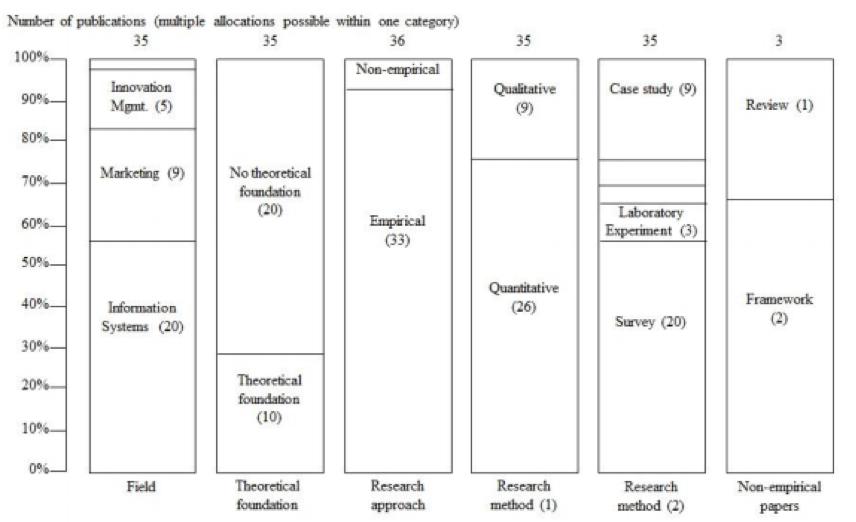
\includegraphics[width=0.8\textwidth]{Picture1.png}
    \caption{Publication diagram}
    \label{fig:mesh1}
\end{figure}

Lorem ipsum dolor sit amet, consetetur sadipscing elitr, sed diam nonumy eirmod tempor invidunt ut labore et dolore magna aliquyam erat, sed diam voluptua. At vero eos et accusam et justo duo dolores et ea rebum. Stet clita kasd gubergren, no sea takimata sanctus est Lorem ipsum dolor sit amet. 
Lorem ipsum dolor sit amet, consetetur sadipscing elitr, sed diam nonumy eirmod tempor invidunt ut labore et dolore magna aliquyam erat, sed diam voluptua. At vero eos et accusam et justo duo dolores et ea rebum. Stet clita kasd gubergren, no sea takimata sanctus est Lorem ipsum dolor sit amet.

\newpage 
\subsection{Yet another sub-section}
As you can see in the figure \ref{fig:mesh1}, everything looks better in a diagram. Also, in the page \pageref{fig:mesh1} 
is the same example.

\newpage\section{Methodology}
Lorem ipsum dolor sit amet, consetetur sadipscing elitr, sed diam nonumy eirmod tempor invidunt ut labore et dolore magna aliquyam erat, sed diam voluptua. At vero eos et accusam et justo duo dolores et ea rebum. Stet clita kasd gubergren, no sea takimata sanctus est Lorem ipsum dolor sit amet. Lorem ipsum dolor sit amet, consetetur sadipscing elitr, sed diam nonumy eirmod tempor invidunt ut labore et dolore magna aliquyam erat, sed diam voluptua. At vero eos et accusam et justo duo dolores et ea rebum. Stet clita kasd gubergren, no sea takimata sanctus est Lorem ipsum dolor sit amet.

\newpage\section{Results}
Lorem ipsum dolor sit amet, consetetur sadipscing elitr, sed diam nonumy eirmod tempor invidunt ut labore et dolore magna aliquyam erat, sed diam voluptua. At vero eos et accusam et justo duo dolores et ea rebum. Stet clita kasd gubergren, no sea takimata sanctus est Lorem ipsum dolor sit amet. Lorem ipsum dolor sit amet, consetetur sadipscing elitr, sed diam nonumy eirmod tempor invidunt ut labore et dolore magna aliquyam erat, sed diam voluptua. At vero eos et accusam et justo duo dolores et ea rebum. Stet clita kasd gubergren, no sea takimata sanctus est Lorem ipsum dolor sit amet.

\subsection{Citation examples}
And here we demonstrate like (\cite{hoehle_espoused_2015}) how citations look alike in this \LaTeX file. You can also list all authors (\cite{venkatesh_usability_2014}). And click any of the references and see what happens in your PDF reader, like here: \cite{university_of_arkansas_mobile_2015}.

\subsection{An example table}
Lorem ipsum dolor sit amet, consetetur sadipscing elitr, sed diam nonumy eirmod tempor invidunt ut labore et dolore magna aliquyam erat, sed diam voluptua. 

\begin{table}[h!]
\centering
\begin{tabular}{|c|c|c|c|} 
 \hline
ID & 1st run & 2nd run & 3rd run \\ [0.5ex] 
 \hline
 1 & 6 & 87837 & 787 \\ 
 \hline
 2 & 7 & 78 & 5415 \\
 \hline
 3 & 545 & 778 & 7507 \\
 \hline
 4 & 545 & 18744 & 7560 \\
 \hline
 5 & 88 & 788 & 6344 \\ 
 \hline
\end{tabular}
\caption{Our amazing results in one, lean table}
\label{table:1}
\end{table}

\newpage
\section{Conclusion}
Lorem ipsum dolor sit amet, consetetur sadipscing elitr, sed diam nonumy eirmod tempor invidunt ut labore et dolore magna aliquyam erat, sed diam voluptua. At vero eos et accusam et justo duo dolores et ea rebum. Stet clita kasd gubergren, no sea takimata sanctus est Lorem ipsum dolor sit amet. Lorem ipsum dolor sit amet, consetetur sadipscing elitr, sed diam nonumy eirmod tempor invidunt ut labore et dolore magna aliquyam erat, sed diam voluptua. At vero eos et accusam et justo duo dolores et ea rebum. Stet clita kasd gubergren, no sea takimata sanctus est Lorem ipsum dolor sit amet. 
 alsdkf jasldfk lsakfdj lsdkf ldsa d sldkf sldk lsdaf lsdakf sdf 

\newpage

%%%%%%%%%%%%%%%%%%%%%%%%%%%%%%%%%%%%%%%%%%%%%%%%%%%%%%%%%%%%%%%%%%%%%%%%%%%%%%%%%%%%%%%%%%%
% "Bibliography" Section
% IMPORTANT: Do not change anything here!
% Add/change your bibliography entries to the "bibliography.bib" file
% Remark: Entries only show up in this section, after you \cite them at least once.
%%%%%%%%%%%%%%%%%%%%%%%%%%%%%%%%%%%%%%%%%%%%%%%%%%%%%%%%%%%%%%%%%%%%%%%%%%%%%%%%%%%%%%%%%%%


\sectionunnumbered{Bibliography}
\pagenumbering{Roman} % set roman page numbers: i, ii, ...
{\linespread{1}\selectfont\printbibliography[heading=none]}

 \newpage

%%%%%%%%%%%%%%%%%%%%%%%%%%%%%%%%%%%%%%%%%%%%%%%%%%%%%%%%%%%%%%%%%%%%%%%%%%%%%%%%%%%%%%%%%%%
% "Appendix" Section
%%%%%%%%%%%%%%%%%%%%%%%%%%%%%%%%%%%%%%%%%%%%%%%%%%%%%%%%%%%%%%%%%%%%%%%%%%%%%%%%%%%%%%%%%%%

\sectionunnumbered{Appendix}
\begin{table}[h!]
\centering
\begin{tabular}{|c|c|c|c|} 
 \hline
Source & 1st run & 2nd run & 3rd run \\ [0.5ex] 
 \hline
 Kentucky & 6 & 87837 & 787 \\ 
 \hline
 California & 7 & 78 & 5415 \\
 \hline
 New Jersey & 545 & 778 & 7507 \\
 \hline
 Manitoba & 545 & 18744 & 7560 \\
 \hline
 Alaska & 88 & 788 & 6344 \\ 
 \hline
\end{tabular}
\caption{Raw data (remark: this one is in the Appendix -> Roman page nr)}
\label{table:raw_data}
\end{table}

\newpage

%%%%%%%%%%%%%%%%%%%%%%%%%%%%%%%%%%%%%%%%%%%%%%%%%%%%%%%%%%%%%%%%%%%%%%%%%%%%%%%%%%%%%%%%%%%
% "Affidavit" Section
%%%%%%%%%%%%%%%%%%%%%%%%%%%%%%%%%%%%%%%%%%%%%%%%%%%%%%%%%%%%%%%%%%%%%%%%%%%%%%%%%%%%%%%%%%%

\sectionunnumbered{Affidavit} 
{I hereby declare that I have developed and written the enclosed seminar thesis entirely on my own and have not used outside sources without declaration in the text. Any concepts or quotations applicable to these sources are clearly attributed to them.\par}
\vspace{0.7cm}
{This seminar thesis has not been submitted in the same or substantially similar version, not even in part, to any other authority for grading and has not been published elsewhere. I am aware of the fact that a misstatement may have serious legal consequences.\par}
\vspace{0.7cm}

% Mannheim,  \titledate\today uncomment this line use date of today automatically
Mannheim, 12. March 2019

\vspace{1.4cm}
Max Mustermann


\end{document}